\documentclass[conference]{IEEEtran}
\IEEEoverridecommandlockouts

\usepackage{cite}
\usepackage{amsmath,amssymb}
\usepackage{graphicx}
\usepackage{booktabs}
\usepackage{multirow}
\usepackage{textcomp}
\usepackage{xcolor}
\usepackage{url}
\usepackage{hyperref}

\def\BibTeX{{\rm B\kern-.05em{\sc i\kern-.025em b}\kern-.08em
    T\kern-.1667em\lower.7ex\hbox{E}\kern-.125emX}}

\begin{document}

\title{Synth Veda: A Two-Stage Routing and Fine-Tuned Transformer Pipeline for Environmental DNA Biodiversity Triage}

\author{
\IEEEauthorblockN{Author Name\IEEEauthorrefmark{1}}
\IEEEauthorblockA{\IEEEauthorrefmark{1}Department/Institution\\
City, Country\\
email@example.com}
}

\maketitle

\begin{abstract}
Environmental DNA (eDNA) sampling produces mixed-organism sequence pools that must be sorted into taxonomic groups, screened for contamination, and checked for signs of undescribed diversity before a survey result means anything to a field biologist. We describe Synth Veda, a working pipeline that routes each sequence to one of six coarse groups (fish, plant, bacteria/pathogen, general animal, human/domestic contamination, and a residual unknown group) using a hand-tuned marker-gene and biophysical heuristic, then classifies within each group using a fine-tuned transformer -- DNABERT-2 for five of the six groups and the Nucleotide Transformer for the group that proved hardest -- into known species, an uncertain taxonomic match, a possible-novelty flag, a possible-contamination flag, or a low-quality flag. On held-out per-route test splits the five easier routes reach 93.6--100\% accuracy (macro F1 0.83--1.00); the bacteria/pathogen route, evaluated after we found and fixed a train/test leakage bug in an earlier version of the dataset, reaches 83.1\% accuracy against an internal 85\% operating target. We report that leakage investigation in full: a sequence-level audit across all six routes shows the earlier duplicate-crossing-splits problem was real but had a measurable accuracy effect of under one point everywhere except the bacteria route, where it had inflated the headline number by roughly 2.5 points. We also describe two supporting subsystems built around the classifiers -- a composite novelty/contamination scorer and a curated, human-reviewed monthly retraining loop with an explicit no-live-update rule -- and are explicit about what remains heuristic rather than learned, including the router itself and the offline field-triage mode.
\end{abstract}

\begin{IEEEkeywords}
environmental DNA, eDNA metabarcoding, DNA barcoding, transformer fine-tuning, DNABERT-2, biodiversity monitoring, data leakage
\end{IEEEkeywords}

\section{Introduction}

A field team running an environmental DNA survey does not get back a tidy list of species. They get a pool of short reads pulled out of water, soil, or sediment, some belonging to the organisms they meant to sample, some belonging to whatever else was in the water at the time -- a passing swimmer, a dog on the shoreline, reagent carryover from the lab -- and, if the site is interesting, a handful of reads that do not match anything in a reference database at all \cite{deiner2017edna,ficetola2008edna,taberlet2012edna}. Turning that pool into something a biologist can act on requires three separate judgments for every read: what kind of organism is this likely to be, is this actually a new observation or a known one, and is this a real signal or contamination. Treating those as one classification problem tends to produce a system that is mediocre at all three.

The approach in this paper splits the problem instead of unifying it. A cheap, deterministic first pass decides which of six broad groups a sequence probably belongs to -- based on which marker-gene region it looks like and simple compositional statistics, not a trained model -- and routes it to a classifier fine-tuned specifically for that group. Within each group, the classifier makes a five-way call: a recognized species, a plausible but uncertain taxonomic match, a candidate for novelty, a candidate for contamination, or a read too degraded to use. That five-way output feeds a second, independent scoring step that combines model confidence, entropy of the class distribution, sequence quality, and a contamination-motif check into a single novelty/contamination signal, because a low-confidence classifier output on its own is a weak basis for calling something a new species.

We built this as a full pipeline, not a benchmark exercise: an API and worker service pair, a MongoDB-backed job and review data model, a curated monthly retraining loop that keeps unvetted user corrections out of the live model, and an offline field-triage mode for surveys run without connectivity. We describe all of it here, but we are careful throughout to separate what has been trained and evaluated against held-out data from what is still rule-based or scaffolding, because a paper that blurs that line is not useful to anyone trying to reproduce or extend the work.

The evaluation results are mixed on purpose -- we are reporting what we measured, not what we hoped for. Five of the six routes perform well by ordinary classification standards. The sixth, bacteria/pathogen classification from 16S-region reads, sits just under an internal 85\% accuracy threshold after two different backbone architectures and a real dataset bug fix, and we discuss why we think that gap reflects a genuinely harder discrimination problem rather than an engineering shortfall. We also describe, in some detail, a train/test leakage bug that inflated an early accuracy number by 2.5 points, because finding it changed how much we trusted every earlier result and because duplicate reference-database records crossing a train/test split is a failure mode that is easy to introduce silently in any project built on public sequence databases.

Our contributions are:
\begin{itemize}
\item A two-stage design -- heuristic marker-gene routing followed by route-specific fine-tuned transformer classification -- for multi-kingdom eDNA triage, together with an honest account of which stage is learned and which is still rule-based.
\item Per-route, per-class evaluation (accuracy, macro F1, precision/recall, confusion matrices) for six fine-tuned classifiers built on two different genomic transformer backbones.
\item A documented train/test leakage investigation: how it was found, how it was fixed for one route, and a follow-up audit quantifying its actual impact on the other five routes, most of which turned out to be only mildly affected.
\item A description of the supporting novelty/contamination scoring, curated-retraining, and offline-mode subsystems, with explicit notes on which parts of each are currently placeholder logic.
\end{itemize}

\section{Related Work}

DNA barcoding -- identifying an organism from a single short, standardized marker region rather than a full genome -- goes back to the proposal that mitochondrial COI could serve as a near-universal animal identifier \cite{hebert2003biological}, with the Barcode of Life Data System (BOLD) established shortly after as the reference repository the field has since converged on \cite{ratnasingham2007bold}. Plant barcoding uses a different marker combination because COI does not vary enough in plants to be useful, settling instead on a matK/rbcL combination \cite{cbol2009plant}, and bacterial community profiling is built almost entirely around 16S rRNA \cite{klindworth201316s}. Fish-specific eDNA metabarcoding has its own dedicated primer sets \cite{miya2015mifish}. This per-kingdom marker specificity is the underlying reason our system routes before it classifies: a single model trained across every marker region at once is trying to learn a much noisier problem than it needs to.

Environmental DNA as a survey method -- detecting species from ambient water, soil, or air rather than from captured specimens -- was demonstrated early for aquatic vertebrates \cite{ficetola2008edna} and has since become a standard biomonitoring tool, reviewed at length elsewhere \cite{deiner2017edna,taberlet2012edna}. That literature is largely concerned with wet-lab protocol and marker choice; it says comparatively little about what happens computationally once the reads come back mixed, low-confidence, and inclusive of sequences that will not match anything in a reference database. That gap is where this paper sits.

On the modeling side, transformer language models pretrained directly on nucleotide sequences -- rather than on hand-engineered k-mer or codon features -- have become the default way to get a general-purpose DNA sequence representation. DNABERT was the first widely adopted example, treating a genome as a sequence of overlapping k-mer tokens and pretraining with a masked-language objective \cite{ji2021dnabert}; DNABERT-2 replaced k-mer tokenization with byte-pair encoding and added architectural changes aimed at cross-species generalization and Windows/GPU-memory-friendlier attention \cite{zhou2023dnabert2}, which is why we use it as our default backbone. The Nucleotide Transformer scales the same basic pretraining recipe to larger parameter counts and a broader multi-species training corpus \cite{dallatorre2023nucleotide}; we use it as an alternative backbone for the one route where DNABERT-2 plateaued short of our accuracy target. Both models descend from the general transformer architecture \cite{vaswani2017attention} and the masked-pretraining-plus-fine-tuning recipe popularized by BERT \cite{devlin2019bert}, applied to a four-letter alphabet instead of natural-language vocabulary. Most published evaluations of these genomic language models target single-organism tasks -- promoter or splice-site prediction in one reference genome, for instance -- rather than a multi-kingdom field triage setting with an explicit unknown/novelty category; we are not aware of published work evaluating this style of model as a route-specific classifier inside a larger routing-and-review pipeline of the kind described here.

\section{System Architecture}

\begin{figure}[t]
\centering
\begin{minipage}{0.48\textwidth}
\footnotesize
\begin{tabular}{@{}l@{}}
\textbf{Upload} (FASTA/JSON) \\
$\downarrow$ \\
\textbf{QC \& parsing} -- length, GC/N ratio, dedup \\
$\downarrow$ \\
\textbf{Heuristic router} -- marker motif + biophysical score \\
\quad$\downarrow$\hspace{2.7em}$\downarrow$\hspace{2.7em}$\downarrow$ \\
\textbf{fish} \quad \textbf{plant} \quad \textbf{...} \quad \textbf{bacteria/path.} \\
(fine-tuned transformer classifier, one per route) \\
$\downarrow$ \\
\textbf{Novelty / contamination scorer} \\
$\downarrow$ \\
\textbf{Report} $\to$ \textbf{human review queue} $\to$ \textbf{monthly curated retrain} \\[0.3em]
\hline \\[-0.9em]
\multicolumn{1}{c}{\emph{(offline: same QC + router + scorer,}}\\
\multicolumn{1}{c}{\emph{no transformer inference, syncs on reconnect)}}
\end{tabular}
\end{minipage}
\caption{Pipeline overview. The routing and scoring stages are rule-based; only the per-route classifiers are learned. The offline field-triage path reuses QC, routing, and scoring but skips transformer inference entirely.}
\label{fig:pipeline}
\end{figure}

Figure~\ref{fig:pipeline} sketches the full pipeline. We describe each stage in turn, and flag explicitly which stages are trained models versus deterministic logic.

\subsection{Heuristic Router}

The router assigns each incoming sequence to one of six routes -- \texttt{fish}, \texttt{plant}, \texttt{bacteria\_pathogen}, \texttt{animal\_general}, \texttt{human\_domestic\_contamination}, or \texttt{misc\_unknown} -- before any transformer runs. It is deliberately not a learned model at this stage. It combines two signal families multiplicatively into a per-route score: an exact-substring check against a small set of conserved marker-region motifs specific to each group's standard barcode (16S for bacteria, COI and the MiFish primer region for fish, rbcL/matK for plants, human mitochondrial and Alu regions for the contamination route) \cite{klindworth201316s,miya2015mifish,cbol2009plant}, and a Gaussian-likelihood score over GC ratio, CpG observed/expected ratio, and sequence length against a hand-set reference profile per route. Scores are normalized into a probability over routes, with a confidence tier (high/medium/low) and a fallback-route list attached to low-confidence calls, and a separate low-quality gate applied before routing based on N-content and length. A sequence's 4-mer frequency profile and a minimizer sketch are computed at this stage for downstream similarity comparisons but are not yet part of the routing score itself.

We are stating plainly that this stage is a heuristic, not a trained classifier, because the natural question is why we did not simply fine-tune one model to do routing and classification together. The answer is that marker-region motif matching is close to definitive when it hits -- a 16S primer match is strong evidence for the bacteria route regardless of what a learned model would say -- and reserving the learned component for the harder within-route decision (known species vs.\ novel vs.\ contaminated vs.\ low-quality) uses the transformer's capacity where cheap heuristics do not already solve the problem.

\subsection{Route-Specific Classification}
\label{sec:routeclassifiers}

Each route has its own fine-tuned classifier: a pretrained transformer backbone plus a linear classification head over the backbone's \texttt{[CLS]}-position embedding, both fine-tuned end to end (no frozen-backbone shortcuts). DNABERT-2-117M \cite{zhou2023dnabert2} is the backbone for five of the six routes. For \texttt{bacteria\_pathogen}, whose 16S-derived reads proved to be the hardest discrimination problem in the whole system, we also trained on the larger Nucleotide Transformer v2-500M backbone \cite{dallatorre2023nucleotide} after DNABERT-2 plateaued below our accuracy target, and report both.

Every route's classifier outputs a label from a shared five-class taxonomy, of which each route uses whichever subset is relevant to its data: \texttt{known\_species}, \texttt{likely\_taxonomic\_group} (a plausible higher-level match without species-level confidence), \texttt{possible\_novelty}, \texttt{possible\_contamination}, and \texttt{low\_quality\_unusable}. A sixth label, \texttt{unknown\_needs\_online\_confirmation}, is reserved for the residual \texttt{misc\_unknown} route and for offline-mode output where a definitive call is deferred until reconnection.

Training uses class-weighted cross-entropy, with weights set by inverse class frequency, because several routes have genuine (not sampling-artifact) class imbalance -- \texttt{likely\_taxonomic\_group} is a rarer real outcome than \texttt{known\_species} for the bacteria route, for instance, and an unweighted loss simply learns to predict the majority class more often. Optimization uses AdamW \cite{loshchilov2019adamw}, 8-bit-quantized for the larger backbone to fit optimizer state in a single consumer-grade GPU's memory budget \cite{dettmers20228bit}, with linear warmup and decay. We track two checkpoint-selection criteria independently through training -- the epoch with lowest validation loss, and the epoch with highest validation accuracy -- and evaluate both against the held-out test set, because committing to one selection criterion up front and never checking whether the other would have generalized better is an easy way to leave measurable performance on the table without ever finding out.

\subsection{Novelty and Contamination Scoring}

A route classifier's raw output is not treated as the final word on novelty. A separate scoring stage combines the classifier's predicted class and confidence with the softmax entropy across all label scores, a sequence-quality signal from QC, an explicit non-contamination gate, and an embedding-based isolation signal, into a single 0--1 novelty score thresholded into none/low/medium/high. The first four signals are genuinely computed from model output and QC metrics; the embedding-isolation signal is currently a placeholder -- a rough norm-based proxy carrying a deliberately small weight in the composite score -- pending a planned future implementation that would compare an embedding against learned per-route cluster centroids. We are naming this rather than quietly shipping it as if it were finished, because a novelty score is only as trustworthy as its least-finished input signal. Contamination flagging runs a parallel combination of the router's own contamination-route signal, motif matching against known lab-reagent and adapter sequences, and biophysical similarity to human/domestic-animal genomic composition.

\subsection{Human-in-the-Loop Curation}

Expert and admin users can confirm, reject, or correct any classifier output, flag possible novelty or contamination directly, and attach supporting evidence, through a review workflow with an explicit state machine (submitted, triaged, needs-evidence, accepted, rejected, duplicate, verified, included-in-training-batch). Corrections do not update any live model. They accumulate in a database and are assembled into a monthly training batch only after review; a new model version is trained on that batch, evaluated against the previous version and a fixed regression set, and promoted only if it does not regress. We treat this as a hard rule rather than a preference, because a pipeline that lets unvetted field corrections retrain a live model in real time is a pipeline that can be quietly poisoned by one persistently wrong or adversarial contributor.

\subsection{Offline Field-Triage Mode}

Surveys run without connectivity -- the motivating case being deep-water or remote sampling -- use a separate offline mode built around a time-boxed, signed offline license issued before departure. Offline analysis runs the same QC and heuristic router described above and the same novelty/contamination scorer, but deliberately does not run transformer inference at all; the route-level and quality signals from QC and routing are enough to support a preserve/resample/continue-sampling recommendation without claiming a species identification the system has not actually computed offline. Every offline action is logged locally and synced for full reanalysis once connectivity returns. Quantized route-specific model packs for genuine offline transformer inference are planned but not yet trained, and we list that explicitly as future work rather than as a shipped capability.

\section{Dataset and Preprocessing}

Training sequences are drawn from two public reference resources: BOLD, the standard barcode-of-life repository \cite{ratnasingham2007bold}, and NCBI's curated nucleotide reference collections, queried through a local BLAST database index \cite{altschul1990blast} rather than downloaded wholesale. Records are mapped from their taxonomic lineage to one of the six routes, then labeled into the five-class taxonomy described in Section~\ref{sec:routeclassifiers} using lineage and organism-name heuristics. Sequences longer than 2{,}000 bases are windowed into overlapping 400-base chunks rather than truncated, so a single long reference record does not either dominate a route's training set or lose the information past a fixed cutoff. Because \texttt{possible\_contamination} is inherently cross-route -- a plant sample contaminated with human DNA is still a plant-route sample -- we inject a controlled fraction of already-collected human/domestic sequences into the plant and bacteria routes specifically, rather than relying on that class occurring naturally in a lineage-based split. Each (route, label) combination is capped during collection so that no single well-represented species or source database can dominate a route's training distribution. Table~\ref{tab:dataset} gives the resulting split sizes per route.

\begin{table}[t]
\centering
\caption{Per-route dataset sizes (sequences).}
\label{tab:dataset}
\begin{tabular}{@{}lrrr@{}}
\toprule
Route & Train & Dev & Test \\
\midrule
fish & 4{,}047 & 505 & 505 \\
plant & 4{,}849 & 606 & 606 \\
animal\_general & 8{,}018 & 1{,}002 & 1{,}002 \\
human\_domestic\_contamination & 4{,}000 & 500 & 500 \\
misc\_unknown & 12{,}000 & 1{,}500 & 1{,}500 \\
bacteria\_pathogen (clean split) & 32{,}865 & 4{,}107 & 4{,}107 \\
\bottomrule
\end{tabular}
\end{table}

\subsection{A Train/Test Leakage Bug, Found and Fixed}
\label{sec:leakage}

While chasing an accuracy plateau on the bacteria/pathogen route, we found that our train/dev/test split had been performed \emph{after} pooling records from multiple reference-database exports, without deduplicating identical sequences first. Public barcode and reference databases legitimately contain near-duplicate or exactly duplicate records -- the same well-characterized species submitted by multiple labs, for instance -- and a naive random split scatters copies of the same sequence across train and test. Splitting the bacteria route's data by sequence identity showed that roughly 13\% of all rows were exact duplicates, and that a meaningful fraction of the test set had a duplicate sitting in the training set. Evaluating the trained model separately on the leaked and genuinely-unseen portions of that test set made the effect concrete: accuracy on sequences the model had already seen during training was 98.6\%, against 82.4\% on sequences it had genuinely never seen, a sixteen-point gap that has only one explanation.

We fixed this for the bacteria route by deduplicating at the sequence level \emph{before} splitting and retraining from scratch on the clean split; that retrained result (Section~\ref{sec:results}) is the one we report and recommend citing. Because the same pooling process was used for the other five routes and none of them had been re-split, we then ran the identical duplicate-membership audit on all six routes rather than assuming the other five were fine simply because no one had gone looking. Table~\ref{tab:leakage} in Section~\ref{sec:results} reports the result: leakage was real everywhere except the bacteria route (which is now clean by construction) and fish (which happened to have none), but its effect on the headline accuracy number was under one point in every other case -- small enough that we do not consider the pre-existing numbers for those five routes materially wrong, unlike the bacteria route where it briefly inflated the headline by roughly 2.5 points.

\section{Evaluation Methodology}

We report accuracy and macro-averaged F1 -- the unweighted mean of per-class F1 scores -- for each route's held-out test split, plus full per-class precision, recall, and F1, and a confusion matrix. Macro averaging is deliberate: several routes have classes with very little test support (a route's \texttt{possible\_novelty} class may have only a handful of examples), and micro/weighted averages would let a route's accuracy on its dominant class hide poor performance on the classes we actually care most about catching. Test splits were held out from training and from checkpoint selection throughout; checkpoint selection used only the validation split described in Section~\ref{sec:routeclassifiers}.

For the leakage audit described in Section~\ref{sec:leakage}, we define a test row as \emph{leaked} if its exact sequence string also appears anywhere in that route's training split, and report accuracy separately on the leaked and non-leaked (``clean'') subsets of each route's test set, using \texttt{scikit-learn}'s standard classification metrics throughout \cite{pedregosa2011sklearn}.

\section{Results}
\label{sec:results}

\begin{table}[t]
\centering
\caption{Per-route test accuracy and macro F1.}
\label{tab:results}
\begin{tabular}{@{}lrrr@{}}
\toprule
Route & Backbone & Acc. & Macro F1 \\
\midrule
fish & DNABERT-2 & 99.80\% & 0.833 \\
plant & DNABERT-2 & 97.03\% & 0.942 \\
animal\_general & DNABERT-2 & 94.71\% & 0.854 \\
human\_domestic\_contam. & DNABERT-2 & 100.00\% & 1.000 \\
misc\_unknown & DNABERT-2 & 93.60\% & 0.935 \\
bacteria\_pathogen & NT-500M & 83.10\% & 0.835 \\
\bottomrule
\end{tabular}
\end{table}

Table~\ref{tab:results} and Figure~\ref{fig:barresults} summarize per-route performance; the bacteria/pathogen number is the clean, post-deduplication result from Section~\ref{sec:leakage}. Five of six routes clear 93\% accuracy, and \texttt{human\_domestic\_contamination} -- a near-binary discrimination between human/domestic and non-human sequence composition -- reaches a perfect 100\% on its test split, which we read as a reflection of how compositionally distinct that split's two classes are rather than as evidence the task is trivial in general. Macro F1 is noticeably lower than accuracy for \texttt{fish} (0.833 despite 99.8\% accuracy) and \texttt{animal\_general} (0.854 against 94.7\% accuracy): both routes have a minority class with single-digit test support, and a model that gets most or all of those few examples wrong drags the unweighted macro average down even though it barely moves overall accuracy. We read this as the macro-F1 metric doing its job, not as a modeling failure -- it is surfacing exactly the class the accuracy number would otherwise hide.

\begin{figure}[t]
\centering
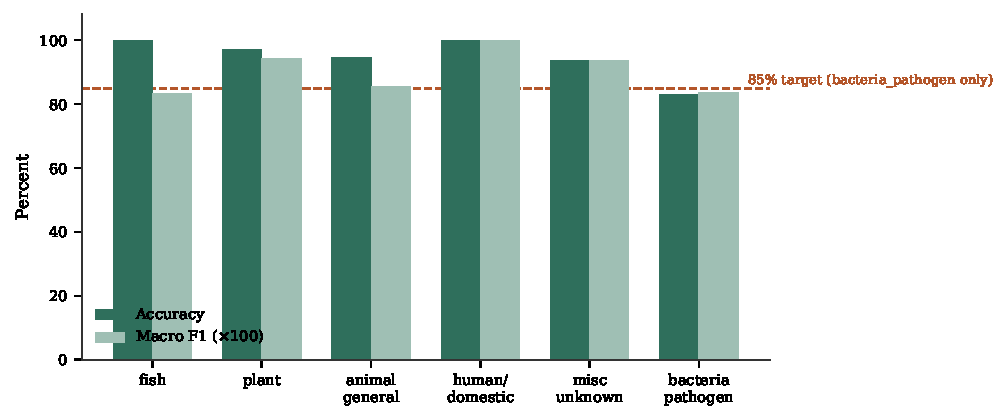
\includegraphics[width=0.49\textwidth]{figures/route_results.pdf}
\caption{Accuracy and macro F1 by route. The dashed line marks the 85\% internal accuracy target that applies specifically to the bacteria/pathogen route.}
\label{fig:barresults}
\end{figure}

\subsection{Bacteria/Pathogen: Two Backbones, One Persistent Gap}
\label{sec:bacteria}

The bacteria/pathogen route -- four-way classification of 16S-region reads into known species, an uncertain higher taxonomic match, possible novelty, or possible contamination -- is the one route that does not clear our internal accuracy target, and it is worth discussing why we think that reflects the task rather than the setup. Figure~\ref{fig:confmat} shows the confusion matrix for the clean-split, dev-loss-selected checkpoint (83.1\% accuracy, 0.835 macro F1). The confusion is concentrated almost entirely between \texttt{known\_species} and \texttt{likely\_taxonomic\_group}: 169 known-species reads are called an uncertain taxonomic match, and 100 uncertain-match reads are called known-species, against comparatively little confusion involving \texttt{possible\_novelty} or \texttt{possible\_contamination}. \texttt{likely\_taxonomic\_group} also has the lowest per-class F1 of the four (0.648, against 0.815--0.987 for the other three), which is consistent with that boundary being the genuinely hard part of the problem rather than a symptom of a mistuned model: at typical 16S amplicon read lengths, the sequence difference between ``this is species X'' and ``this is somewhere in X's genus but I cannot commit to the species call'' can be a handful of variable-region bases, and no amount of additional model capacity changes how much information is actually present in the input.

That last point is why we tried a second, larger backbone rather than only re-tuning the first one. Moving from DNABERT-2-117M to the Nucleotide Transformer at roughly 4.3$\times$ the parameter count, and roughly six to seven times the training wall-clock time on our hardware, bought a 0.3-point accuracy improvement over DNABERT-2's best clean-split result -- a real but modest gain, not the qualitative jump that would suggest the earlier backbone was simply too small for the task. We take that as evidence the \texttt{known\_species}/\texttt{likely\_taxonomic\_group} boundary is close to its information-theoretic ceiling at this read length and marker choice, rather than evidence that a still-larger model would close the remaining 1.4--1.9 points to our target.

\begin{figure}[t]
\centering
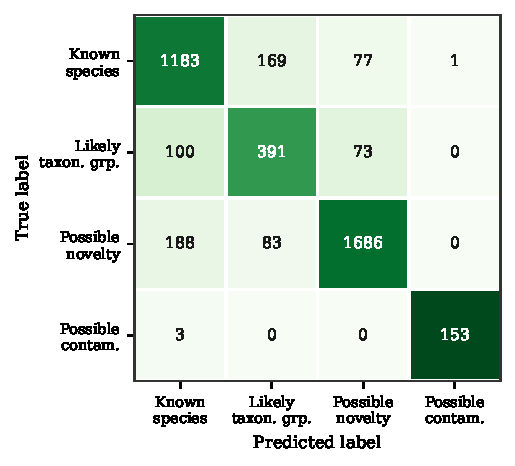
\includegraphics[width=0.46\textwidth]{figures/confusion_bacteria.pdf}
\caption{Confusion matrix, bacteria/pathogen route, clean split (Nucleotide Transformer, dev-loss-selected checkpoint). Cell shading is row-normalized; cell values are raw counts.}
\label{fig:confmat}
\end{figure}

\subsection{Leakage Audit Across All Six Routes}

\begin{table}[t]
\centering
\caption{Train/test leakage audit, all routes.}
\label{tab:leakage}
\begin{tabular}{@{}lrrrr@{}}
\toprule
Route & Leaked & Headline & Clean-only & $\Delta$ \\
\midrule
fish & 0.0\% & 99.80\% & 99.80\% & 0.00 \\
plant & 3.8\% & 97.03\% & 96.91\% & 0.12 \\
animal\_general & 17.1\% & 94.71\% & 93.74\% & 0.97 \\
human\_domestic\_contam. & 1.8\% & 100.00\% & 100.00\% & 0.00 \\
misc\_unknown & 5.1\% & 93.60\% & 93.33\% & 0.27 \\
bacteria\_pathogen$^{*}$ & 0.0\% & 83.10\% & 83.10\% & 0.00 \\
\bottomrule
\multicolumn{5}{l}{\footnotesize $^{*}$Rebuilt with sequence-level deduplication (Section~\ref{sec:leakage}).}
\end{tabular}
\end{table}

Table~\ref{tab:leakage} reports the audit described in Section~\ref{sec:leakage} applied to all six routes rather than only the one where the problem was first noticed. The \texttt{animal\_general} route has the highest leakage rate of any route by percentage -- 17.1\% of its test rows have a duplicate in training, higher than the bacteria route's original problem -- yet its headline-to-clean accuracy gap is under one point, well short of the sixteen-point leaked-versus-clean gap the bacteria route showed. We read this difference as evidence that leakage's actual damage depends on how hard the underlying task already is: on a task the model generalizes well on regardless, seeing a few memorized duplicates in the test set barely moves the number, whereas on a genuinely difficult discrimination the same duplicates can substitute memorization for generalization and meaningfully overstate performance. Three routes (\texttt{plant}, \texttt{human\_domestic\_contamination}, \texttt{misc\_unknown}) show measurable but small leakage with no practical accuracy effect. We consider the headline numbers for those three, and for \texttt{animal\_general}, defensible as reported, while treating the sub-one-point clean-only figures in the table as the more rigorous number where that level of scrutiny matters.

\section{Discussion and Limitations}

We are stating our limitations plainly rather than folding them into future-work language, because several of them bear directly on how much weight the results above should carry.

\textbf{The router is heuristic, not learned.} Marker-motif matching and biophysical scoring work well when a sequence clearly matches one route's expected signature, and degrade gracefully to a fallback-route list when it does not, but the routing stage has no learned component and no way to improve from data the way the downstream classifiers do. Replacing it with a learned embedding-based router is planned future work, not a solved problem.

\textbf{One novelty-scoring signal is a placeholder.} The embedding-isolation component of the composite novelty score is currently a weak proxy carrying a small, deliberately limited weight, pending a planned implementation based on learned per-route cluster centroids. We flag this because a novelty score is a claim researchers may act on, and we would rather understate its current sophistication than have it read as more finished than it is.

\textbf{Offline mode does not run the trained classifiers at all.} It is a genuine limitation, not a compressed or quantized version of the online pipeline: field-triage recommendations offline are based on QC and routing signals alone, explicitly without a species-level classification, and results are labeled as requiring confirmation once connectivity returns.

\textbf{Results reflect single training runs.} We did not train multiple random seeds per route and report variance; the numbers in Section~\ref{sec:results} are single-run results, and some of the differences discussed here (particularly the sub-point deltas in Table~\ref{tab:leakage}) are close enough to plausible run-to-run noise that they should be read as indicative rather than exact.

\textbf{Training data comes from curated reference databases, not field samples.} Every result in this paper is measured against held-out splits of BOLD and NCBI reference records. We have not yet evaluated the pipeline against raw eDNA reads from an actual field survey, which typically carry degradation, chimeric artifacts, and a different contamination profile than curated database records do; we expect some accuracy drop under that distribution shift and are not in a position to quantify it yet.

\textbf{The bacteria/pathogen gap is, on current evidence, a hard-task ceiling rather than a fixable bug.} We say this carefully: it is possible that more or better-curated 16S training data, a longer amplicon window, or a different marker region entirely would close the remaining gap to our 85\% target, and we do not want to overstate the case that it cannot be closed. What the two-backbone comparison in Section~\ref{sec:bacteria} rules out, we think, is that simply scaling up model capacity on the current data and read length is the fix.

\section{Conclusion and Future Work}

Synth Veda routes environmental DNA reads through a cheap heuristic classifier into six taxonomic groups and then applies a fine-tuned transformer specific to each group, reaching 93.6--100\% accuracy on five routes and 83.1\% on the sixth against an internal target of 85\%. Along the way we found and fixed a genuine train/test leakage bug, and rather than quietly moving on once the one affected route was fixed, we audited all six routes for the same problem and report that most were only mildly affected -- a result we think is worth publishing precisely because it is not the dramatic finding we initially expected once we knew where to look.

The most immediate next steps are the ones we have flagged as limitations rather than as finished work: replacing the heuristic router with a learned, embedding-based one; finishing the cluster-centroid novelty signal; evaluating against real field-collected reads rather than only reference-database splits; and running multi-seed training to put honest error bars on the numbers in Table~\ref{tab:results}. On the bacteria/pathogen route specifically, we intend to test whether a longer amplicon window or additional curated 16S training data closes the remaining gap before concluding that 83--85\% is the practical ceiling for this task at this read length.

\bibliographystyle{IEEEtran}
\bibliography{references}

\end{document}
